\documentclass{article}

\usepackage[english]{babel}
\usepackage{authblk}
\usepackage[a4paper,top=2cm,bottom=2cm,left=3cm,right=3cm,marginparwidth=1.75cm]{geometry}
\usepackage{amsmath}
\usepackage{graphicx}
\usepackage{gensymb}
\usepackage{textcomp}
\usepackage[backend=biber, style=nature]{biblatex}
\usepackage{csquotes}
\usepackage[toc,page]{appendix}
\usepackage[colorlinks=true, allcolors=blue]{hyperref}
\usepackage{multirow}
\usepackage{tabularx}

\addbibresource{references.bib}

\title{Predicting Ensemble Location and Width in Binaural Recordings of Music with Convolutional Neural Networks}
\author[1,*]{Paweł Antoniuk}
\author[1]{Sławomir Zieliński}
\affil[1]{Faculty of Computer Science, Białystok University of Technology}
\affil[*]{Corresponding author: pawel.antoniuk@sd.pb.edu.pl}
\date{}

\begin{document}
\maketitle


\begin{abstract}
  Binaural audio technology has been in existence for many years, but its popularity has significantly increased over the past decade as a consequence of advancements in virtual reality and streaming technologies. Along with its growing popularity, the quantity of publicly accessible binaural audio materials has also expanded. Consequently, there is now a need for automated and objective measurements of spatial content information, with ensemble location and width being the most prominent. This study presents a novel method for predicting ensemble location and width in binaural recordings. To this end, 30 head-related transfer functions and 192 binaural music recordings from publicly accessible multi-track recording repositories were used to synthesize 23,040 binaural recordings. The synthesized recordings were then used to train a multi-task convolutional neural network model, the aim of which was to predict the location and width of the ensemble for unseen recordings. The results indicate that models of ensemble location and width can be successfully constructed with low prediction errors --- $4.76\degree$ ($\pm0.10\degree$) for ensemble location and $8.57\degree$ ($\pm0.19\degree$) for ensemble width. The method developed in this study outperforms previous spatiogram-based methods recently published in the literature and holds promise for future development as a part of a novel tool for audio engineers to assess binaural audio.
\end{abstract}

\section{Introduction}

The human auditory system demonstrates exceptional proficiency in segregating, localizing, and interpreting diverse auditory signals, despite being limited to two ears. This capability arises from the intricate analysis of temporal, amplitude, and spectral disparities, a process termed binaural hearing \cite{blauert_spatial_1996}, which enables precise localization of sound sources in complex auditory environments. An important advantage of binaural hearing is demonstrated by the `cocktail party effect', which showcases the system's capacity to concentrate on individual sounds while suppressing background noise \cite{cherry_experiments_1953}. An understanding of the auditory system is essential for comprehending its limits and creating more immersive binaural experiences for entertainment purposes \cite{zhang_surround_2017}. It also helps to improve hearing aid devices by enhancing auditory signal reception and improving spatial awareness \cite{hirsh_binaural_1950, thiemann_speech_2016}.

The advancement of sophisticated machine learning techniques, particularly deep learning networks, has spurred an intriguing exploration into the extent to which these tools can emulate the human auditory system. This exploration proceeds without reliance on the advanced spatial audio feature engineering traditionally used in audio source localization, as evidenced by references \cite{yang_deepear_2022, vera-diaz_towards_2018, pang_multitask_2019}. While the application of convolutional neural networks (CNNs) \cite{lecun_handwritten_1989} to audio signals --- especially in conjunction with spectrograms \cite{thomas_analyzing_2014, espi_exploiting_2015} or other techniques \cite{abdel-hamid_applying_2012, sainath_deep_2013} --- is not novel, it has been successfully employed in prior studies. Building on these foundations, this study developed an audio localization method by creating a multi-task CNN model.

Inspired by the fact, that humans tend to localize sound sources in groups rather than individually \cite{bregman_auditory_1990, rumsey_spatial_2002}, the objective of the proposed model is to predict ensemble location and width instead of positions of individual sources. This study is unique as it not only conceptualized the method but also tested it on a vast, real-life music corpus of 23,040 binaural excerpts that were synthesized using 192 multi-track music recordings and 30 publicly available head-related transfer functions (HRTFs) from various sources. The music recordings encompassed various genres, including rock, jazz, pop, and classical music.

The findings demonstrate that this method is effective in accurately predicting the spatial characteristics of sound sources in near-real-world scenarios. Furthermore, this paper presents an experiment framework that allows for the objective measurement of a binaural localization technique in an objective manner, utilizing a large-scale dataset synthesized from real-world examples of music signals (for other use cases for this framework, see \cite{antoniuk2023blind, zielinski_automatic_2022, zielinski_spatial_2022, zielinski_comparison_2020}). One of the key advantages of the proposed method is that it does not assume the number of audio sources. However, a significant limitation of this study is the lack of reverberation in the synthesized recordings, which represents a material for future research.

The developed method has the potential to be highly beneficial in automated assessment tasks, where a significant number of binaural recordings must be evaluated and labeled in terms of their spatial content information. This may assist audio engineers in objectively assessing and segregating binaural audio recordings with regard to their spatial content. Furthermore, it could facilitate the development of an autonomous web-crawler bot that will collect binaural recordings from publicly accessible repositories and label them according to the spatial properties of the sound sources, such as the location of the music ensemble or the sparsity of audio source positions.

The remainder of this paper is organized as follows: Section \ref{sec:related-studies} presents related studies. The description of the method developed for this study is provided in Section \ref{sec:methodology}, which also includes detailed definitions of ensemble location and width, along with a description of the experiments used to evaluate this method. Section \ref{sec:results} discusses the results of the method-evaluation experiments conducted in this study. Finally, the paper concludes in Section \ref{sec:conclusions}.

\section{Related studies}
\label{sec:related-studies}

The majority of existing literature on the subject of sound source localization employs techniques that leverage the advantages of microphone arrays with more than two channels \cite{kaveh_statistical_1986, pavlidi_real-time_2012, pan_multi-tone_2021, hahmann_sound_2022, chung_sound_2022, liu_sound_2022}. In the context of sound source localization in binaural signals, the predominant focus of research is on the identification of individual sound sources, rather than groups of sounds \cite{dietz_auditory_2011, may_probabilistic_2011, may_binaural_2012, woodruff_binaural_2012, may_robust_2015, ma16c_interspeech, ma_exploiting_2017, benaroya_binaural_2018}. In terms of source direction of arrival (DOA) methods, the majority of research assumes a fixed number of sound sources \cite{pang_multitask_2019, vecchiotti19, ma_exploiting_2017, woodruff_binaural_2012, s_spatiogram_2021}, which limits its practical applications as this information is rarely known in real-life binaural recordings. Moreover, the majority of studies have focused on relatively homogeneous signals, namely speech \cite{dietz_auditory_2011, may_probabilistic_2011, may_binaural_2012, woodruff_binaural_2012, may_robust_2015, ma16c_interspeech, ma_exploiting_2017, benaroya_binaural_2018, wang_binaural_2020, liu_multiple_2018, yang_deepear_2022, ma_robust_2018}.

In contrast to the aforementioned studies, the proposed method is not constrained by the number of sources. Furthermore, the approach is not limited to speech and has been applied to a wide range of musical datasets, including instruments and vocals. In contrast to previous studies that primarily focused on individual sources, the proposed method does not aim to separate them, but rather considers them as a group, or in this case, a musical ensemble. This approach is similar to how the real musical ensembles are arranged on stage, thereby emphasizing practical applications in live settings. To the authors' knowledge, this is one of the first methods to localize ensemble width (see \cite{antoniuk2023blind} for the previous ensemble-width-related study), and the first to localize both ensemble position and width simultaneously using a multi-task model.


Sound localization methods can be classified into two categories based on the implementation of their underlying algorithms: glass-box (e.g., \cite{dietz_auditory_2011, may_probabilistic_2011, may_binaural_2012, may_robust_2015, woodruff_binaural_2012, ma16c_interspeech, ma_exploiting_2017, ma_robust_2018}) and black-box (e.g., \cite{vecchiotti19, vera-diaz_towards_2018, yang_deepear_2022}). Glass-box methods, more traditional in the literature, rely on manually designed algorithms that mimic the auditory system to explicitly extract key features for location prediction, such as interaural level differences, interaural time differences, interaural coherence, or interaural phase differences (see \cite{blauert_spatial_1996} for feature descriptions). An example of one of the most advanced auditory models that is able to extract such features was developed by the Two!Ears project \cite{raake_computational_nodate}.

In contrast, black-box methods generally employ minimal feature engineering, relying instead on advanced machine learning techniques to autonomously extract features and make predictions. These methods, while effective, do not explicitly reveal the features they extract nor necessarily mimic the human auditory system. This opacity and the unpredictable nature of the outcomes, coupled with their dependency on deep neural networks that have extensive learning parameters, require the use of very large datasets for development and evaluation. Such datasets often include thousands of examples, as seen in the TIMIT corpus with 6300 examples \cite{garofolo_john_s_timit_1993} used in multiple studies \cite{yang_deepear_2022, benaroya_binaural_2018, wang_binaural_2020, vecchiotti19, ma_exploiting_2017, pang_multitask_2019, ma_robust_2018, may_robust_2015}, or custom corpora comprising hundreds of thousands of recordings \cite{antoniuk2023blind, zielinski_automatic_2022, zielinski_spatial_2022, zielinski_comparison_2020}. This poses a significant challenge in assembling a sufficiently large and diverse collection of labeled binaural recordings. However, this challenge can be addressed through the synthesis of binaural sounds, as demonstrated in various studies \cite{antoniuk2023blind, zielinski_automatic_2022, zielinski_spatial_2022, zielinski_comparison_2020,yang_deepear_2022, ma_robust_2018} and further elaborated upon in Section \ref{subsec:synthesis} of this paper.

\section{Methodology}
\label{sec:methodology}

This section presents a detailed description of the main objective of the model developed as part of this study, as outlined in Section \ref{subsec:ensemble_definition}. It also describes the audio dataset used for training and evaluating the model, as detailed in Section \ref{subsec:synthesis}. In Section \ref{subsec:feature_extraction}, the feature extraction procedure is presented. Section \ref{subsec:topology} describes the model topology, whereas Section \ref{subsec:training_evaluation} address model training and evaluation.

\subsection{Ensemble location and width definition}
\label{subsec:ensemble_definition}

The objective of the model developed in this study is to predict the ensemble location ($\theta$) and width ($\omega$), as illustrated in Figure \ref{fig:scene}. An ensemble is defined as a group of audio point sources positioned on a circle around the listener on a virtual acoustic scene with equal distance to the listener. The location of source $i$ is denoted by $\theta_i$. The ensemble width ($\omega$) is defined as the angular width between two extreme point sources ($max_i(\theta_i)-min_i(\theta_i)$), while the ensemble location, designated by $\theta$, represents the middle angle between two extreme sound sources ($(max_i(\theta_i)+min_i(\theta_i))/2$). For the purposes of this study, the locations of the sources were limited to the frontal hemisphere only, i.e. $\theta\in[-45\degree, 45\degree]$, $\omega\in[0\degree, 90\degree]$, as this range encompasses the majority of real-world recording scenarios. It should be noted that although humans possess some limited abilities to localize sound sources in the vertical plane, in this study all sources are placed in the horizontal plane, at the height of the listener. This covers the majority of cases for real-world recordings (see \cite{ma_robust_2018, zielinski_spatial_2022} for similar studies that cover top-down discrimination).

\begin{figure}[ht]
  \centering
  \includegraphics[width=\linewidth]{../pictures/scene.png}
  \caption{\label{fig:scene}Illustration of ensemble width ($\omega$) and ensemble location ($\theta$) that are relative to the direction of the head. Black dots represent the positions of audio sources $\theta_i$. The ensemble location ($\theta$) is defined as the angular position of the center of the ensemble relative to the direction the head is turned. The ensemble width ($\omega$) is defined as angular distance between two extreme audio sources. }
\end{figure}

\subsection{Synthesis of binaural music recordings}
\label{subsec:synthesis}

The experiments conducted in this study involved 23,040 binaural recordings of music. The binaural recordings were synthesized using 192 multi-track publicly-available music recordings \cite{noauthor_mixing_nodate} and 30 HRTF databases (see Table \ref{table:hrtfs} in \nameref{appendix:a_hrtf} for a detailed list of HRTF databases used in this study). The number of tracks in multi-track recording ranged from 5 to 62, with median of 9. For each pair of a multi-track recording and an HRTF database, four binaural recordings were synthesized with different random ensemble parameters, namely location $\theta$ and width $\omega$, as defined in Section \ref{subsec:ensemble_definition}. Both parameters were drawn from a uniform random distribution. Furthermore, the tracks of the input multi-track recordings were randomly assigned to sound source positions ($\theta_i$) to enhance the diversity of the final binaural corpora. Before the synthesis, the tracks were equalized to $-23$ LUFS, in accordance with the ITU-R BS.1770 recommendation \cite{noauthor_recommendation_nodate}.

The binaural recordings were obtained in this study using the binaural synthesis procedure, known as binauralization, whose aim was to simulate the positions of sound sources within a virtual acoustic environment \cite{blauert_spatial_1996}. This was achieved by convolving multi-track signals with head-related impulse responses from a specified head-related transfer function (HRTF) database. The resulting binaural output signal $y_c[n]$ for each stereo channel $c$ (left or right) at sample $n$ is given by the following equation:
\begin{equation}
  y_c[n] = \sum_{i=1}^{N} \sum_{k=0}^{K-1} x_i[k] \times h_{c,\theta_i}[n-k] ,
\end{equation}
where $x_i$ represents the signal of an individual sound source $i$ from the input music recording and $h_{c,\theta_i}$ denotes the head-related impulse response for channel $c$ at location $\theta_i$ of source track $i$.

Due to copyright restrictions, the music corpus utilized in this study was not published and can be provided upon request to the authors of this paper.

\subsection{Feature extraction}
\label{subsec:feature_extraction}

% The procedure proposed in this study did not 

% Zamiast tego dac obrazek z glowami i spektrogramami, lewy i prawi i roznica, sprawdzic czy to ma sens, potencjalnie usunac
% \begin{figure}[ht]
%   \centering
%   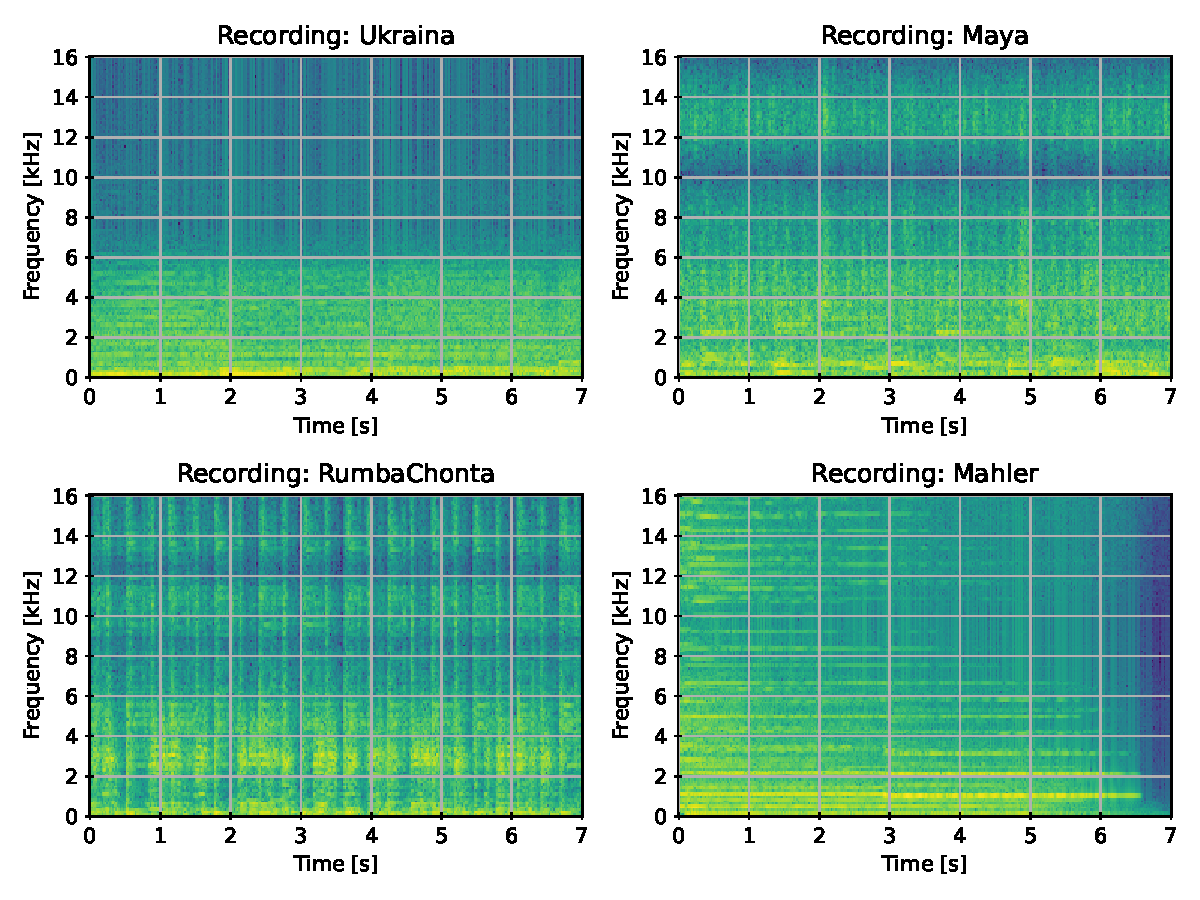
\includegraphics[width=\linewidth]{../figures/samples.pdf}
%   \caption{\label{fig:samples}Example magnitude spectrograms from randomly selected synthesized binaural music recordings, used as input data for training and evaluating the convolutional neural network (CNN) in this study. }
% \end{figure}

% Figure \ref{fig:samples} displays example spectrograms from four distinct binaural recordings, exhibiting a broad bandwidth and the diversity of the signals used in this study

Prior to input into the model, the binaural recordings of music were transformed into magnitude spectrograms. It is important to note that the original spectrograms were preserved in a floating-point precision matrix format, which prevented any loss of information due to precision conversion. The spectrograms were calculated using the Fast Fourier Transform (FFT) algorithm, with a limitation of 150 bands, spaced linearly from 100 Hz to 16 kHz. Additionally, a Hamming window of 40 ms was applied to each frame of the signal, resulting in a total of 349 time frames. This procedure was conducted for both the left and right channels, yielding two spectrograms for each binaural sample. Each sample was represented by a matrix of dimensions $2 \times 349 \times 150$. This method parallels the procedure presented in \cite{zielinski_automatic_2022}.

\subsection{Network topology}
\label{subsec:topology}

\begin{figure}[ht]
  \centering
  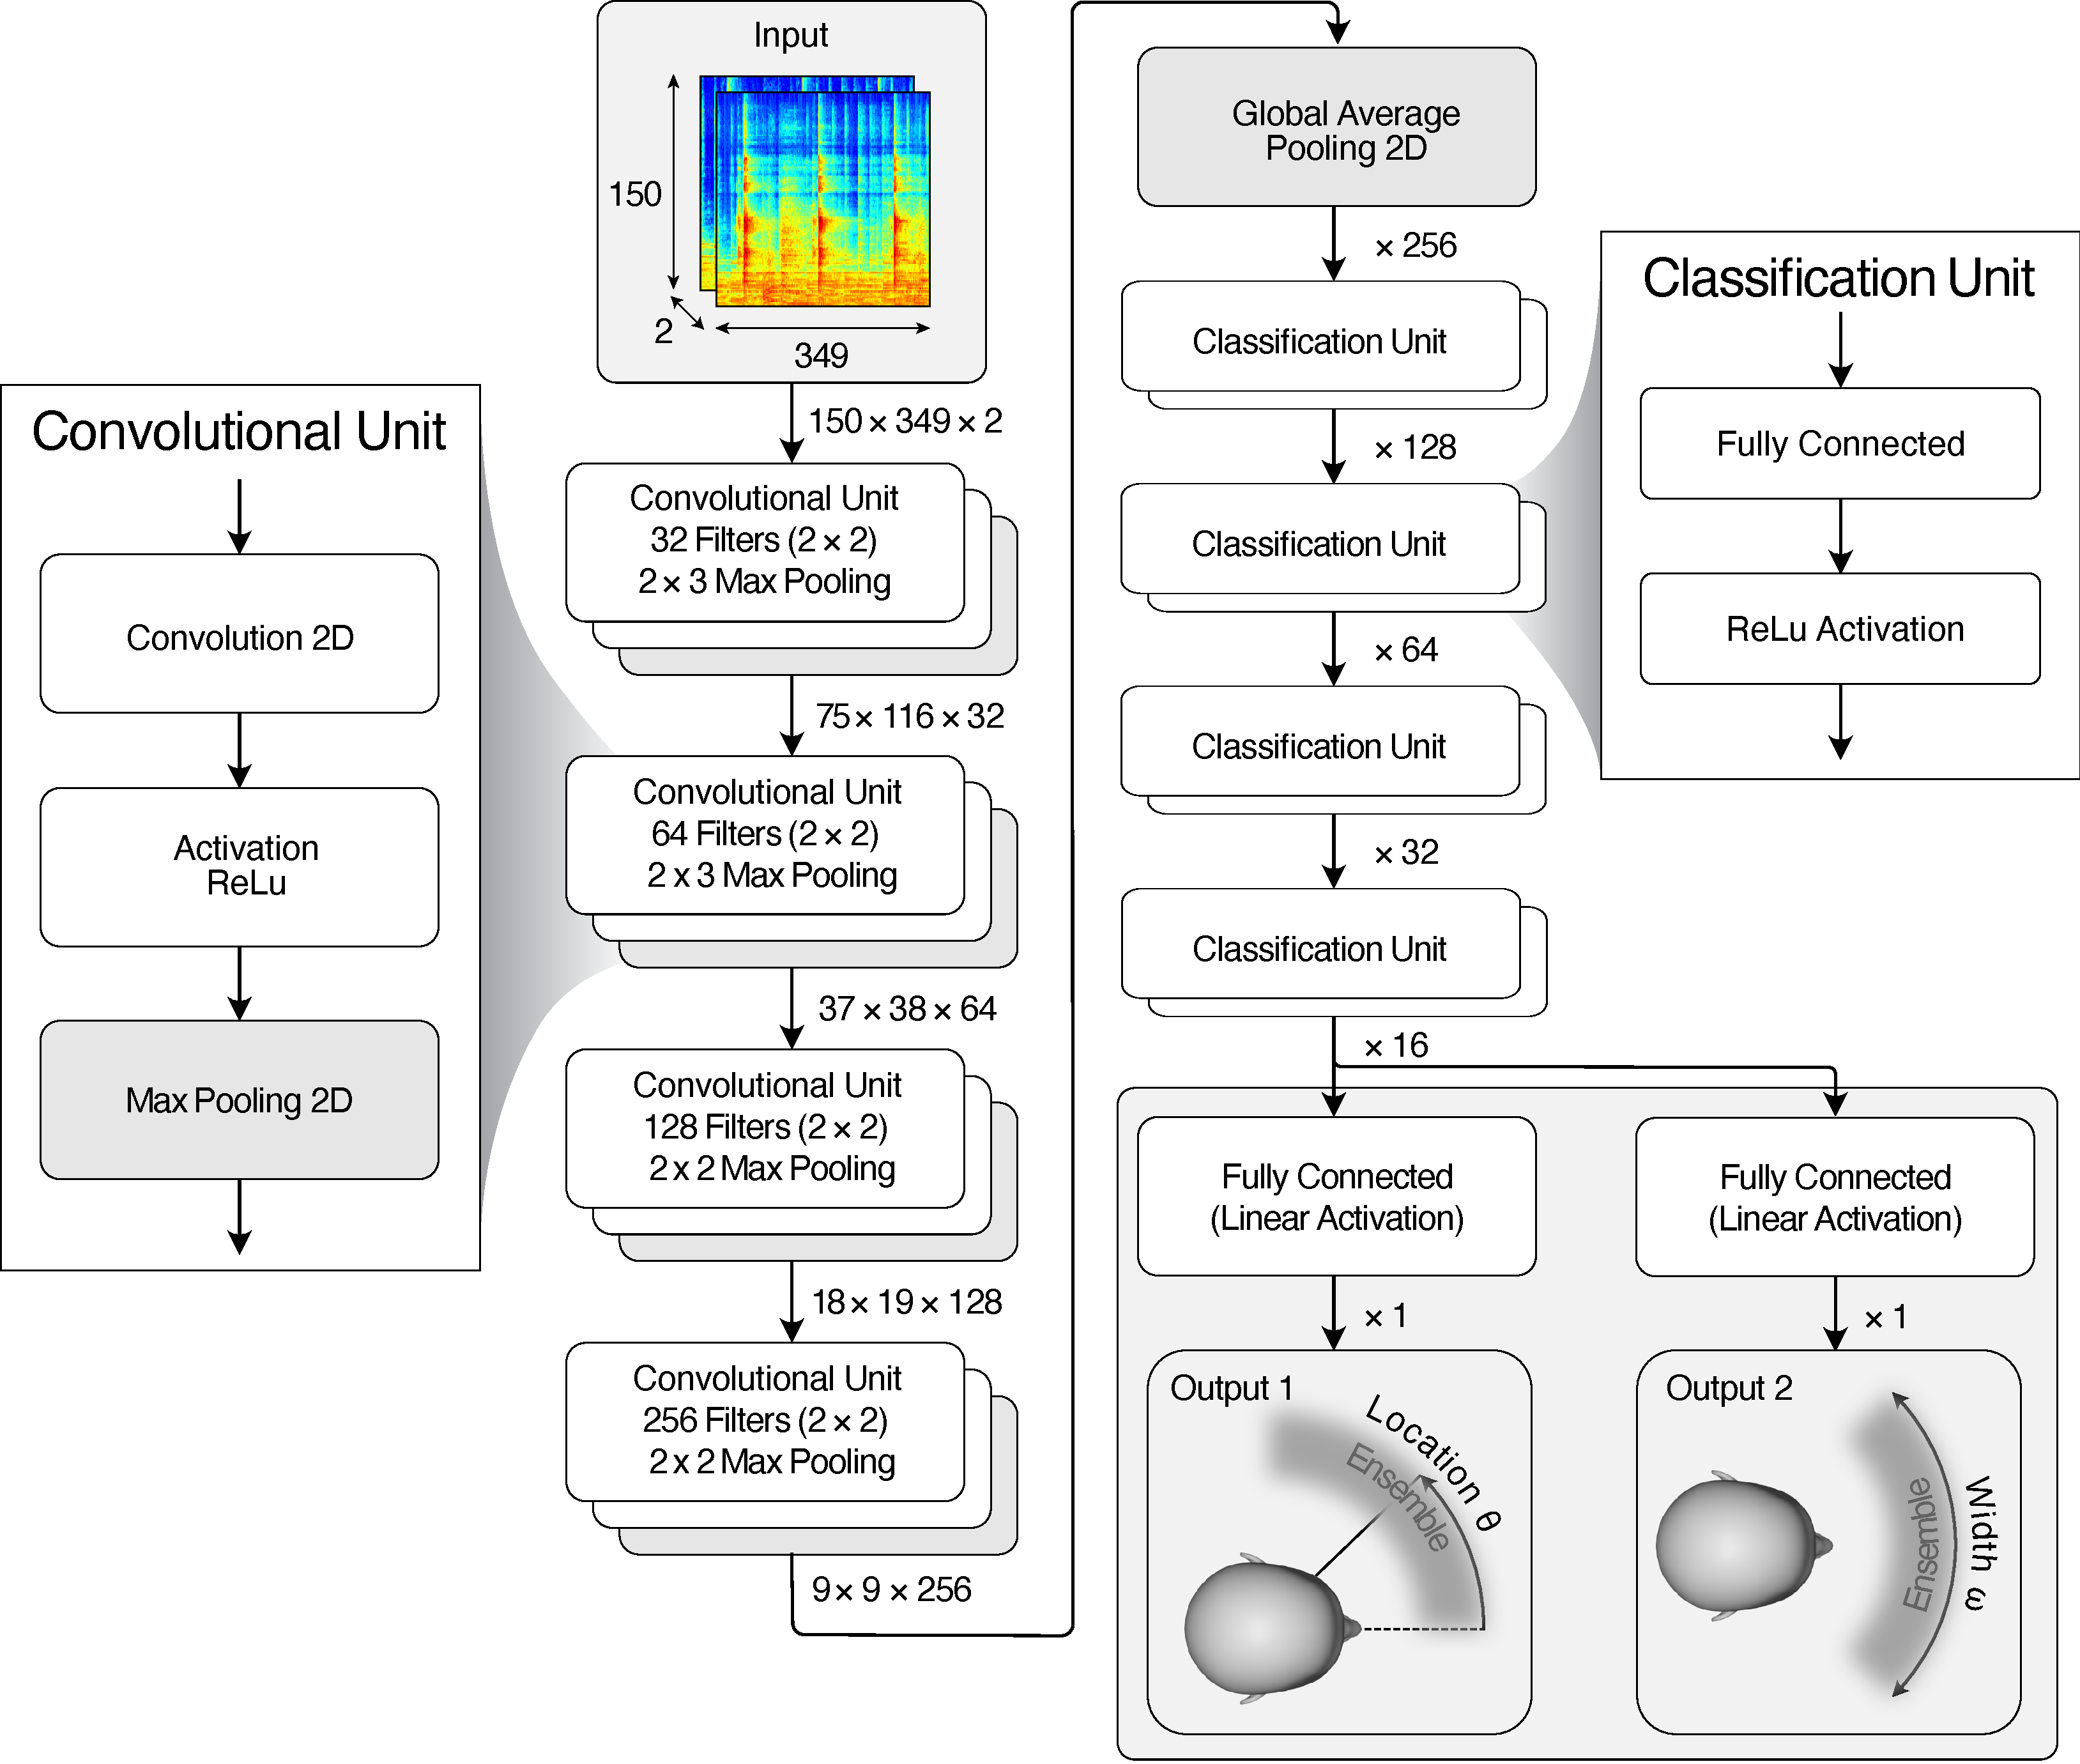
\includegraphics[width=\linewidth]{../pictures/architecture.pdf}
  \caption{\label{fig:architecture}Topology of the Convolutional Neural Network (CNN) used for identifying ensemble location and width}
\end{figure}

The network topology employed in this study, depicted in Figure \ref{fig:architecture}, was significantly influenced by the AlexNet convolutional neural network \cite{krizhevsky_imagenet_2012}. Although AlexNet was originally designed for image classification, this study adapted it for the audio prediction task by converting binaural recordings into magnitude spectrograms, as described in Section \ref{subsec:feature_extraction}. This conversion allowed the spectrograms to be treated as images, enabling their use in a standard image-prediction-like task.

The network accepts two spectrograms as inputs, and its architecture consists of a series of convolutional units followed by classification units, culminating in two output heads for predicting ensemble width and location. The architecture was designed in a multi-task fashion, enabling a single network to predict both ensemble parameters simultaneously. This multi-task capability is achieved by connecting the output of the final classification unit to two separate outputs, one for each ensemble parameter.

Despite the availability of widely used techniques for addressing overfitting, such as the Dropout Layer \cite{srivastava_dropout_nodate}, and for accelerating training, such as Batch Normalization \cite{ioffe_batch_2015}, neither technique was employed in this study due to their observed ineffectiveness for the specific prediction task at hand. Instead, a Global Average Pooling Layer \cite{lin_network_2014} was utilized, known for its proven capabilities in reducing overfitting. In this particular task, the inclusion of this layer significantly reduced overfitting, lowering the final mean absolute error score by $0.83\degree$ (average across 10 trials) compared to configurations using a Flattening Layer.


\subsection{Model training and evaluation}
\label{subsec:training_evaluation}

Monte-Carlo cross validation (without replacement).

\section{Results}
\label{sec:results}

\begin{figure}[ht]
  \centering
  \begin{minipage}[t]{0.45\linewidth}
    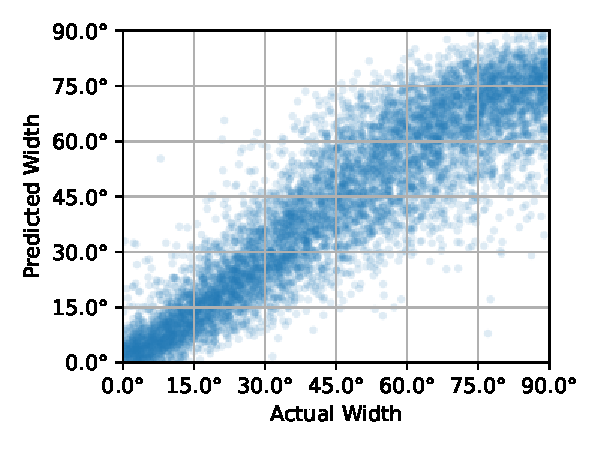
\includegraphics[width=\linewidth]{../figures/actual_vs_predicted_width.pdf}
    \caption{\label{fig:actual_vs_predicted_width}A comparison between the actual ensemble width $\omega$ and the predicted ensemble width $\omega'$ for a single iteration (of the total five) }
  \end{minipage}
  \hspace{0.5cm}
  \begin{minipage}[t]{0.45\linewidth}
    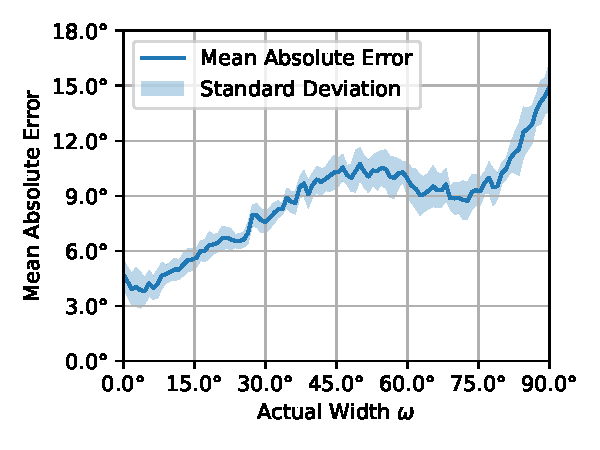
\includegraphics[width=\linewidth]{../figures/mae_width.pdf}
    \caption{\label{fig:mae_width}The impact of the actual ensemble width $\omega$ on the mean absolute prediction error, averaged across all five iterations, with indicated standard deviation.}
  \end{minipage}
\end{figure}

Figure \ref{fig:actual_vs_predicted_width} illustrates the comparison between the actual and predicted ensemble widths. The results demonstrate that the model exhibits better prediction quality for narrower ensemble widths ($5.65^\circ$ for $\omega < 30^\circ$) and that its performance deteriorates with an increase in ensemble width ($12.44^\circ$ for $\omega > 80^\circ$). This suggests that the actual ensemble width significantly impacts the accuracy of ensemble width estimation, leading to worse predictions as width increases. Figure \ref{fig:mae_width} further demonstrates that the relationship between the error and the width is not linear, exhibiting an interesting depression between $60^\circ$ and $75^\circ$.

\begin{figure}[ht]
  \centering
  \begin{minipage}[t]{0.45\linewidth}
    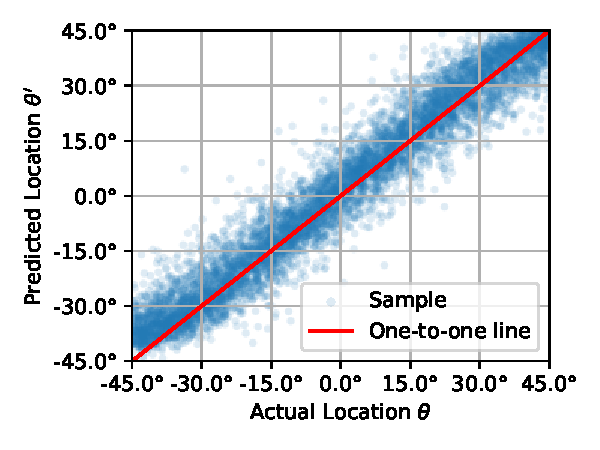
\includegraphics[width=\linewidth]{../figures/actual_vs_predicted_location.pdf}
    \caption{\label{fig:actual_vs_predicted_location}A comparison between the actual ensemble location $\theta$ and the predicted ensemble location $\theta'$ for a single iteration (of the total five) }
  \end{minipage}
  \hspace{0.5cm}
  \begin{minipage}[t]{0.45\linewidth}
    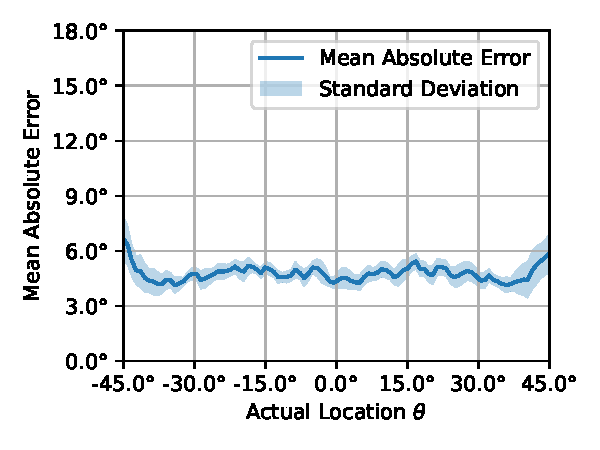
\includegraphics[width=\linewidth]{../figures/mae_location.pdf}
    \caption{\label{fig:mae_location}The impact of the actual ensemble width $\omega$ on the mean absolute prediction error, averaged across all five iterations, with indicated standard deviation.}
  \end{minipage}
\end{figure}

In contrast to the correlation between ensemble width and its prediction error, there is no significant relationship between the actual location and its prediction error, as illustrated in Figures \ref{fig:actual_vs_predicted_location} and \ref{fig:mae_location}. This finding indicates that the model's capabilities for localizing the center of the ensemble is robust, unaffected by the actual spatial positioning of the ensemble, including lateral locations.

% jak uzyskane wyniki koresponduja z literatura: w jjednym przypadku ejst lepsza niz metoda oparta na spatiogramach, a w drugim przypadku nie ma 
The mean absolute prediction error for ensemble width was $8.57^\circ$ ($\pm0.19^\circ$), while the error for ensemble location prediction was $4.76^\circ$ ($\pm0.10^\circ$). Although both ensemble parameters were constrained within the same angular span of $90^\circ$, the ensemble location was predicted with significantly better precision --- approximately $80\%$ better. This shows that the model prediction quality is much better for ensemble location prediction than width prediction. This difference can be attributed to the fact that the model's performance on ensemble width deteriorates significantly for wider ensembles, whereas location prediction remains largely unaffected. For a visual comparison, please refer to Figures \ref{fig:mae_location} and \ref{fig:mae_width}.

\begin{figure}[ht]
  \centering
  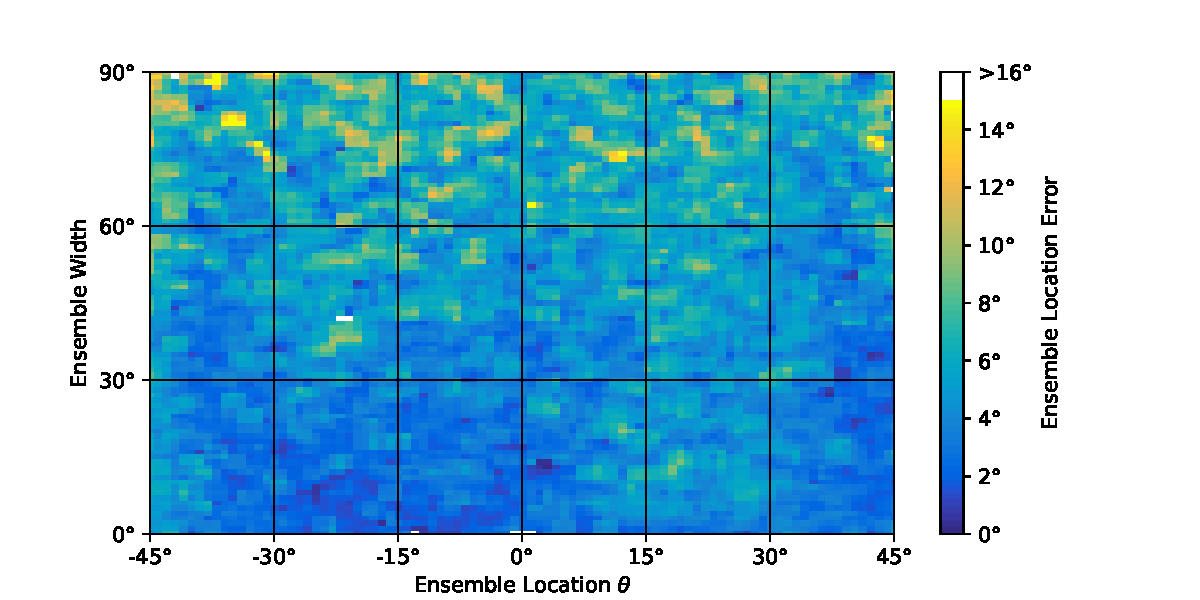
\includegraphics[width=\linewidth]{../figures/map_mae_location.pdf}
  \caption{\label{fig:map_mae_location}The heatmap that illustrates the mean absolute error (MAE) of ensemble location distribution across different ensemble locations (x-axis) and ensemble widths (y-axis). The color intensity corresponds to the MAE values, with lighter areas indicating higher errors.}
\end{figure}

\begin{figure}[ht]
  \centering
  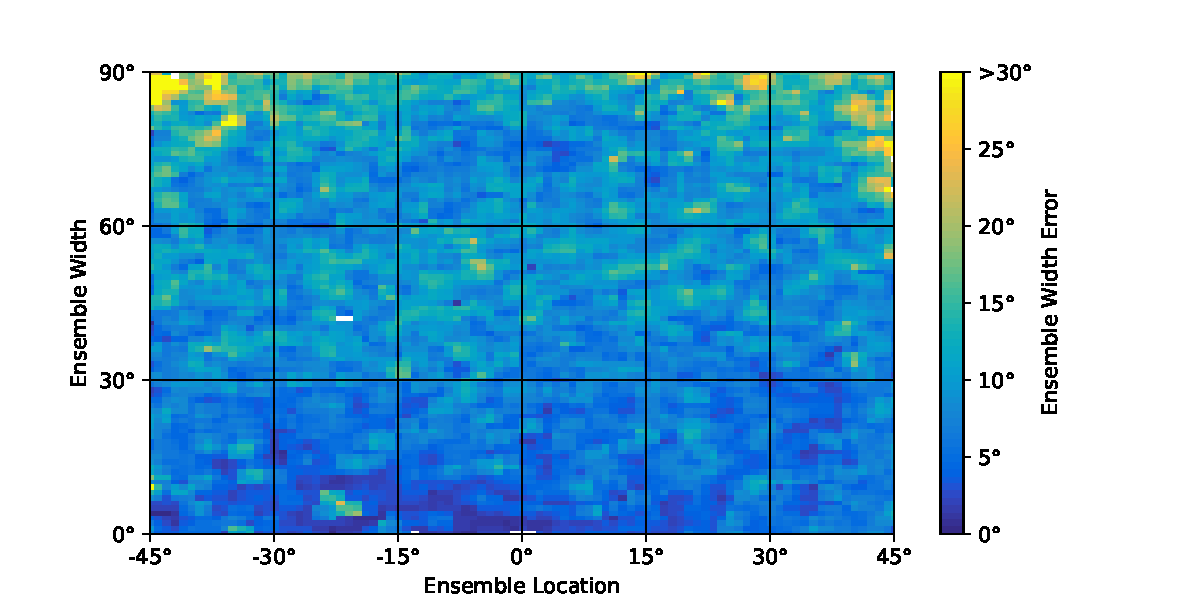
\includegraphics[width=\linewidth]{../figures/map_mae_width.pdf}
  \caption{\label{fig:map_mae_width}The heatmap that illustrates the mean absolute error (MAE) of ensemble width distribution across different ensemble locations (x-axis) and ensemble widths (y-axis). The color intensity corresponds to the MAE values, with lighter areas indicating higher errors. Notably, the values between $30\degree$ and $60\degree$ on the y-axis exhibit unexpectedly higher MAE values region --- please see Figure \ref{fig:mae_width} for comparison. }
\end{figure}

Figure \ref{fig:map_mae_location} illustrates the influence of both ensemble location and width on the mean absolute error for ensemble location, offering a detailed view complementing the results presented in Figure \ref{fig:mae_location}. Some asymmetric anomalies are depicted in this figure, mostly within the $\theta \in [15\degree, 30\degree]$ region, which can be attributed to the sparsity of sample result data across this heatmap. Although this figure primarily shows that ensemble location does not significantly influence the model's location prediction accuracy, it does demonstrate that ensemble width has a significant impact. Similarly, Figure \ref{fig:map_mae_width} reveals a characteristic depression in $\omega \in [30\degree, 60\degree]$ previously shown from a different perspective in Figure \ref{fig:mae_width}. This heatmap highlights another interesting phenomenon in its upper corners --— the error in these areas is considerably higher. This indicates that the model's performance for estimating ensemble width is substantially worse at extreme widths and locations, i.e., when both the width and locations are at their maximum.

\section{Conclusions}
\label{sec:conclusions}

% 1. napisac wnioski, potem occulusion. we wnioskach odniesc sie do spatiogramach

\clearpage
\section*{Appendix A}
\label{appendix:a_hrtf}

{\renewcommand{\arraystretch}{1.1}
\begin{table}[!h]
  \begin{center}
    \caption{\label{table:hrtfs}List of HRTF sets used to synthesize binaural audio excerpts}
    \begin{tabularx}{\linewidth}{
      |>{\hsize=0.3\hsize}X|
      >{\hsize=0.7\hsize}X|
      >{\raggedright\hsize=1.3\hsize}X|
      >{\raggedright\hsize=0.6\hsize}X|
      >{\raggedright\arraybackslash\hsize=2.1\hsize}X|
      >{\hsize=1\hsize}X|
      }
      \cline{1-6}
      \textbf{No.} & \textbf{Type} & \textbf{Head}                             & \textbf{Radius {[}m{]}} & \textbf{Source}                                                                                                                                             & \textbf{Acronym}                \\
      \cline{1-6}
      1.           & Human         & Human subject                             & 1.2                     & \multirow{2}{\hsize}{RWTH Aachen University \cite{braren_high-resolution_2020}}                                                                             & \multirow{2}{\hsize}{AACHEN}    \\
      \cline{1-4}
      2.           & Artificial    & GRAS 45BB-4 KEMAR                         & 1                       &                                                                                                                                                             &                                 \\
      \cline{1-6}
      3.           & Human         & Subject 2                                 & 1.2                     & \multirow{4}{\hsize}{Austrian Academy of Sciences \cite{noauthor_hrtf-database_nodate}}                                                                     & \multirow{4}{\hsize}{ARI}       \\
      \cline{1-4}
      4.           & Human         & Subject 4                                 & 1.2                     &                                                                                                                                                             &                                 \\
      \cline{1-4}
      5.           & Human         & Subject 10                                & 1.2                     &                                                                                                                                                             &                                 \\
      \cline{1-4}
      6.           & Artificial    & ARI Printed Head                          & 1.2                     &                                                                                                                                                             &                                 \\
      \cline{1-6}
      7.           & Human         & Subject 012                               & 1                       & \multirow{3}{\hsize}{CIPIC Interface Laboratory, University of California \cite{algazi_cipic_2001}}                                                         & \multirow{3}{\hsize}{CIPIC}     \\
      \cline{1-4}
      8.           & Human         & Subject 015                               & 1                       &                                                                                                                                                             &                                 \\
      \cline{1-4}
      9.           & Human         & Subject 020                               & 1                       &                                                                                                                                                             &                                 \\
      \cline{1-6}
      10.          & Artificial    & Neumann KU 100                            & 0.9                     & NASA (2007) \cite{andreopoulou_inter-laboratory_2015}                                                                                                       & \multirow{2}{\hsize}{CLUBFRITZ} \\
      \cline{1-6}
      11.          & Artificial    & Neumann KU 100                            & 1.5                     & Helsinki University of Technology (2009) \cite{andreopoulou_inter-laboratory_2015}                                                                          &                                 \\
      \cline{1-6}
      12.          & Artificial    & FABIAN                                    & 1.47                    & \multirow{4}{\hsize}{Technical University Berlin, Huawei Technologies, Munich Research Centre, Sennheiser Electronic \cite{brinkmann_cross-evaluated_2019}} & \multirow{4}{\hsize}{HUTUBS}    \\
      \cline{1-4}
      13.          & Human         & Subject pp2                               & 1.47                    &                                                                                                                                                             &                                 \\
      \cline{1-4}
      14.          & Human         & Subject pp3                               & 1.47                    &                                                                                                                                                             &                                 \\
                   &               &                                           &                         &                                                                                                                                                             &                                 \\
      \cline{1-6}
      15.          & Human         & Subject 1003                              & 1.95                    & \multirow{2}{\hsize}{IRCAM, AKG \cite{noauthor_listen_2023}}                                                                                                & \multirow{2}{\hsize}{LISTEN}    \\
      \cline{1-4}
      16.          & Human         & Subject 1002                              & 1.95                    &                                                                                                                                                             &                                 \\
      \cline{1-6}
      17.          & Artificial    & KEMAR DB-4004 (DB-061)                    & 1.4                     & \multirow{2}{\hsize}{MIT \cite{gardne_hrtf_1994}}                                                                                                           & \multirow{2}{\hsize}{MIT}       \\
      \cline{1-4}
      18.          & Artificial    & KEMAR DB-4004 (DB-065)                    & 1.4                     &                                                                                                                                                             &                                 \\
      \cline{1-6}
      19.          & Human         & Subject 001                               & 1.5                     & \multirow{3}{\hsize}{Tohoku University \cite{watanabe_dataset_2014}}                                                                                        & \multirow{3}{\hsize}{RIEC}      \\
      \cline{1-4}
      20.          & Human         & Subject 002                               & 1.5                     &                                                                                                                                                             &                                 \\
      \cline{1-4}
      21.          & Artificial    & Koken SAMRAI                              & 1.5                     &                                                                                                                                                             &                                 \\
      \cline{1-6}
      22.          & Artificial    & Neumann KU 100                            & 1.2                     & \multirow{3}{\hsize}{University of York \cite{armstrong_perceptual_2018}}                                                                                   & \multirow{3}{\hsize}{SADIE II}  \\
      \cline{1-4}
      23.          & Human         & Subject H3                                & 1.2                     &                                                                                                                                                             &                                 \\
      \cline{1-4}
      24.          & Human         & Subject H4                                & 1.2                     &                                                                                                                                                             &                                 \\
      \cline{1-6}
      25.          & Artificial    & KEMAR                                     & 1                       & South China University of Technology \cite{yu_near-field_2018}                                                                                              & SCUT                            \\
      \cline{1-6}
      26.          & Artificial    & Neumann KU 100                            & 1                       & TH Köln  \cite{porschmann_spherical_2017}                                                                                                                   & TH Köln                         \\
      \cline{1-6}
      27.          & Artificial    & FABIAN                                    & 1.7                     & \multirow{2}{\hsize}{TU Berlin \cite{brinkmann_high_2017, wierstorf_free_2011}}                                                                             & \multirow{2}{\hsize}{TU Berlin} \\
      \cline{1-4}
      28.          & Artificial    & GRAS 45BA KEMAR                           & 1                       &                                                                                                                                                             &                                 \\
      \cline{1-6}
      29.          & Artificial    & GRAS 45BB-4 KEMAR - subject A attachment  & 1                       & \multirow{3}{\hsize}{Aalborg University; University of Iceland \newline \cite{spagnol_viking_2019,spagnol_viking_2020}}                                     & \multirow{3}{\hsize}{VIKING}    \\
      \cline{1-4}
      30.          & Artificial    & GRAS 45BB-4 KEMAR - subject B attachments & 1                       &                                                                                                                                                             &                                 \\
                   &               &                                           &                         &                                                                                                                                                             &                                 \\
      \cline{1-6}
    \end{tabularx}
  \end{center}
\end{table}

\printbibliography

\end{document}

